% This file was converted to LaTeX by Writer2LaTeX ver. 1.0.2
% see http://writer2latex.sourceforge.net for more info
\documentclass[twoside,letterpaper]{article}
\usepackage[latin1]{inputenc}
\usepackage[T1]{fontenc}
\usepackage[english]{babel}
\usepackage{amsmath}
\usepackage{amssymb,amsfonts,textcomp}
\usepackage{color}
\usepackage{array}
\newcolumntype{M}[1]{>{\centering\arraybackslash}m{#1}}
\usepackage{supertabular}
\usepackage{hhline}
\usepackage{hyperref}
\usepackage{float}
\hypersetup{pdftex, colorlinks=true, linkcolor=blue, citecolor=blue, filecolor=blue, urlcolor=blue, pdftitle=SOFTWARE DESIGN DOCUMENT (SRS), pdfauthor=Shaylyn Adams}
\usepackage[pdftex]{graphicx}
% Outline numbering
\setcounter{secnumdepth}{5}
\renewcommand\thesection{\arabic{section}}
\renewcommand\thesubsection{\arabic{section}.\arabic{subsection}}
\renewcommand\thesubsubsection{\arabic{section}.\arabic{subsection}.\arabic{subsubsection}}
\renewcommand\theparagraph{\arabic{section}.\arabic{subsection}.\arabic{subsubsection}.\arabic{paragraph}}
\renewcommand\thesubparagraph{\arabic{section}.\arabic{subsection}.\arabic{subsubsection}.\arabic{paragraph}.\arabic{subparagraph}}
\makeatletter
\newcommand\arraybslash{\let\\\@arraycr}
\makeatother
% Page layout (geometry)
\setlength\voffset{-1in}
\setlength\hoffset{-1in}
\setlength\topmargin{0.5in}
\setlength\oddsidemargin{1in}
\setlength\evensidemargin{1in}
\setlength\textheight{8.278in}
\setlength\textwidth{6.5in}
\setlength\footskip{0.561in}
\setlength\headheight{0.5in}
\setlength\headsep{0.461in}
% Footnote rule
\setlength{\skip\footins}{0.0469in}
\renewcommand\footnoterule{\vspace*{-0.0071in}\setlength\leftskip{0pt}\setlength\rightskip{0pt plus 1fil}\noindent\textcolor{black}{\rule{0.25\columnwidth}{0.0071in}}\vspace*{0.0398in}}
% Pages styles
\makeatletter
\newcommand\ps@Standard{
  \renewcommand\@oddhead{\selectlanguage{english}\rmfamily\color{black} University of Massachusetts CICS \hfill \hfill Health-e}
  \renewcommand\@evenhead{\@oddhead}
  \renewcommand\@oddfoot{\foreignlanguage{english}{\textcolor{black}{SDD Page }}\foreignlanguage{english}{\textcolor{black}{\thepage{}}}}
  \renewcommand\@evenfoot{\@oddfoot}
  \renewcommand\thepage{\arabic{page}}
}
\newcommand\ps@Convertviii{
  \renewcommand\@oddhead{}
  \renewcommand\@evenhead{\@oddhead}
  \renewcommand\@oddfoot{}
  \renewcommand\@evenfoot{\@oddfoot}
  \renewcommand\thepage{\arabic{page}}
}
\newcommand\ps@Convertvii{
  \renewcommand\@oddhead{}
  \renewcommand\@evenhead{\@oddhead}
  \renewcommand\@oddfoot{}
  \renewcommand\@evenfoot{\@oddfoot}
  \renewcommand\thepage{\arabic{page}}
}
\newcommand\ps@Convertvi{
  \renewcommand\@oddhead{}
  \renewcommand\@evenhead{\@oddhead}
  \renewcommand\@oddfoot{}
  \renewcommand\@evenfoot{\@oddfoot}
  \renewcommand\thepage{\arabic{page}}
}
\newcommand\ps@Convertv{
  \renewcommand\@oddhead{}
  \renewcommand\@evenhead{\@oddhead}
  \renewcommand\@oddfoot{}
  \renewcommand\@evenfoot{\@oddfoot}
  \renewcommand\thepage{\arabic{page}}
}
\newcommand\ps@Convertiv{
  \renewcommand\@oddhead{}
  \renewcommand\@evenhead{\@oddhead}
  \renewcommand\@oddfoot{}
  \renewcommand\@evenfoot{\@oddfoot}
  \renewcommand\thepage{\arabic{page}}
}
\newcommand\ps@Convertii{
  \renewcommand\@oddhead{}
  \renewcommand\@evenhead{\@oddhead}
  \renewcommand\@oddfoot{}
  \renewcommand\@evenfoot{\@oddfoot}
  \renewcommand\thepage{\arabic{page}}
}
\newcommand\ps@FirstPage{
  \renewcommand\@oddhead{}
  \renewcommand\@evenhead{\@oddhead}
  \renewcommand\@oddfoot{}
  \renewcommand\@evenfoot{\@oddfoot}
  \renewcommand\thepage{\arabic{page}}
}
\makeatother
\pagestyle{Standard}
\setlength\tabcolsep{1mm}
\renewcommand\arraystretch{1.3}
% footnotes configuration
\makeatletter
\renewcommand\thefootnote{\arabic{footnote}}
\makeatother
\begin{document}
\clearpage\setcounter{page}{1}\pagestyle{Standard}
\thispagestyle{FirstPage}
\clearpage{\centering\selectlanguage{english}\bfseries\color{black}
SOFTWARE DESIGN DOCUMENT (SDD) FOR 
\par}


\bigskip

{\centering\selectlanguage{english}\bfseries\color{black}
320 Green Team Project
\par}


\bigskip


\begin{figure}
\centering

\includegraphics[width=1.5in,height=1.5in]{Uma_seal.png}
\end{figure}

\bigskip


\bigskip

{\centering\selectlanguage{english}\bfseries\color{black}
Version 1.0
\par}

{\centering\selectlanguage{english}\bfseries\color{black}
November 13, 2015
\par}


\bigskip


\bigskip

{\centering\selectlanguage{english}\bfseries\color{black}
Prepared for:
\par}

{\centering\selectlanguage{english}\bfseries\color{black}
Sunderland/Leverett, MA Health Inspector
\par}


\bigskip


\bigskip

{\centering\selectlanguage{english}\bfseries\color{black}
Prepared by:
\par}

{\centering\selectlanguage{english}\bfseries\color{black}
Ather Akhtar, Andrew Chang, Peter Marathas, Andrew Marchetti, \par} 
{\centering\selectlanguage{english}\bfseries\color{black}
 Michael Markman, Eric Maryea, Neven Recchia,
\par}
{\centering\selectlanguage{english}\bfseries\color{black}
Shawn Sowersby, Alex Sullivan, and Josh Tranfaglia.\par}

{\centering\selectlanguage{english}\bfseries\color{black}
University of Massachusetts
\par}

{\centering\selectlanguage{english}\bfseries\color{black}
Amherst, MA \ 01003
\par}


\clearpage{\centering\selectlanguage{english}\bfseries\color{black}
\foreignlanguage{english}{\MakeUppercase{\ }}\foreignlanguage{english}{\MakeUppercase{320 
Green Team Project: Health-e}}
\par}

{\centering\selectlanguage{english}\bfseries\color{black}
TABLE OF CONTENTS
\par}


\bigskip

{\selectlanguage{english}\bfseries\color{black}
Section\ \hfill  Page}

\setcounter{tocdepth}{9}
\renewcommand\contentsname{}
\tableofcontents

\bigskip

\clearpage\section[INTRODUCTION]{\selectlanguage{english}\rmfamily\bfseries\color{black}
INTRODUCTION}
The purpose of this software design document is to provide a low-level description of Health-e, providing insight into the structure and design of each component. In short, this document is meant to equip the reader with a concrete understanding of the inner workings of the Health-e system.

\subsection[GOALS \& OBJECTIVES]{\selectlanguage{english}\rmfamily\bfseries\color{black}
GOALS \& OBJECTIVES}
{\selectlanguage{english}\rmfamily\color{black}
The purpose of Health-e is to replace the current physical method of archiving Board of Health data from restaurant inspections, well reports, and septic tank reports with a new, digital system. The intended user of the tablet aspect of this product is a health inspector who will be using the tablet to document or browse for data while on sight at an inspection. Accordingly, the final product must be quick, efficient, and easy to use. It must offer the appropriate features to the user without overwhelming them or requiring them to spend valuable time learning how to use said features. The user interface should be intuitive and easy to learn so that the system acts as a tool for the user, not something that slows them down while they are doing their job.
}

\subsubsection[Browsing and Search]{\selectlanguage{english}\rmfamily\bfseries\color{black}
Browsing and Search}
{\selectlanguage{english}\rmfamily\color{black}
The user must be able to quickly and efficiently find the data that they are searching for on the tablet. This requires a streamlined browsing and search interface that allows the user to visualize results in an easy-to-read manner. They will be able to enter a search query into a search bar that will always exist in the same location on the page, and results will be displayed in a list format with the most relevant results at the top. The focus here is that the user should not have to spend time searching through the list of results to find the data they are looking for; maneuvering through the results should be a quick, intuitive process.  
}
\subsubsection[Form Entry]{\selectlanguage{english}\rmfamily\bfseries\color{black}
Form Entry}
{\selectlanguage{english}\rmfamily\color{black}
Form entries should model the paper version of the forms in which the inspector would normally fill out on location. They will not replicate the paper forms exactly since that would cause the user to have to constantly zoom in and out on the tablet to fill in sections of the form due to the size of a typical tablet screen. Rather, all fields that appear on the paper forms will appear on the tablet forms in a simple, clean format. The user interface here should be predictable and exist in the natural, chronological order in which the inspector would typically fill out the fields so that it is efficient and easy to use. 
}
\subsubsection[Delayed Upload]{\selectlanguage{english}\rmfamily\bfseries\color{black}
Delayed Upload}
{\selectlanguage{english}\rmfamily\color{black}
The user should not have to have a second thought about delayed upload. That being said, the system must effectively notify the user of the current status of certain documents. Having an icon system that identifies documents on the tablet as being uploaded or in queue for delayed upload will allow the user to remain in the loop as far as the status of their documents in a simple, noninvasive manner.
}

\clearpage\subsection[PROJECT OVERVIEW \& SCOPE]{\selectlanguage{english}\rmfamily\bfseries\color{black}
PROJECT OVERVIEW \& SCOPE}
{\selectlanguage{english}\rmfamily\color{black}
The Health-e system is comprised of two main user components: a web app and a tablet app. For the sake of this design document, we will only be focusing on the tablet app portion of this system. Within this document, the terms user and health inspector will be interchangeable as they are one in the same for this project. The following are some definitions of common phrases that will be used in this document.
}

\begin{flushleft}
\tablehead{}
\begin{supertabular}{|m{1.3587599in}|m{5.00806in}|}
\hline
\centering \selectlanguage{english}\bfseries\color{black} Term or
Acronym &
\centering\arraybslash \selectlanguage{english}\bfseries\color{black}
Definition\\\hline
\selectlanguage{english}\color{black} UML &
\selectlanguage{english}\color{black} Unified Modeling Language\\\hline

\selectlanguage{english}\color{black} DFD &
\selectlanguage{english}\color{black} Data Flow Diagram\\\hline
\selectlanguage{english}\color{black} SDD &
\selectlanguage{english}\color{black} Software Design Document, aka SDS,
Software Design Specification\\\hline
\selectlanguage{english}\color{black} SRS &
\selectlanguage{english}\color{black} Software Requirements
Specification\\\hline

\end{supertabular}
\end{flushleft}

\subsubsection{Core features}
{\selectlanguage{english}\rmfamily\color{black}
The tablet app will include the following core features:
\begin{enumerate}
\item User Authentication
\begin{itemize}
\item Asks the user for their unique password to ensure that the information stored on the tablet app is safe and secure
\end{itemize}
\item Form Entry
\begin{itemize}
\item Streamlines the form entry process by providing all necessary fields in a clean, organized format
\item Provides restaurant, well, and septic forms available to choose from with ease
\item Replicates the original forms in terms of color coding, field names, and information
\end{itemize}
\item Location Entry
\begin{itemize}
\item Documents the current location of the user in terms of coordinates
\item Maps the user's location and their proximity to other septic tanks and wells in the area
\end{itemize}
\item Browsing and Search
\begin{itemize}
\item Allows the user to complete a search query using the search bar
\item Displays search results in a scrolling list form that is easy to maneuver through
\item Displays search results in a variety of orders depending on the user's specification
\newline\newline
\end{itemize}
\item Form Printing
\begin{itemize}
\item Displays what a form will appear as on a printed page with options to print or cancel
\end{itemize}
\item Delayed Upload
\begin{itemize}
\item Categorizes completed forms as either uploaded or pending for delayed upload
\item Displays to the user which forms fall in which category based on icons associated with the forms
\end{itemize}
\end{enumerate}
}

\subsubsection{Addtional features}
{\selectlanguage{english}\rmfamily\color{black}
Below are some features that are not guaranteed to be incorporated in the final product, but could potentially be included, time permitting. Due to their tentative nature, they will not be covered in this document.
\begin{enumerate}
\item Accessibility
\begin{itemize}
\item The user could be able to change certain accessibility options such as form layout, background customization, and font size or style
\end{itemize}
\item Device Synchronization
\begin{itemize}
\item The user could be able to synchronize data across multiple devices such as tablets and mobile devices
\end{itemize}
\end{enumerate}
}

\subsection[SOFTWARE CONTEXT]{\selectlanguage{english}\rmfamily\bfseries\color{black}
SOFTWARE CONTEXT}
{\selectlanguage{english}\rmfamily\color{black}
Health-e will ideally be made available on both the Android and iOS market free of charge. Development and maintenance costs are essentially nonexistent, so funding will not be an issue. The final product will exist under the confines of this course and future extensions to the product, while possible, will probably not be taken up by the group currently implementing this product, if at all. 
\newline\newline Of the core features mentioned above, only the \textit{Form Entry}, \textit{Browsing and Search}, and \textit{Delayed Upload} features will be discussed further in this document as those are the only features that the Green Team will be focusing on for this project. 
}

\subsection[MAJOR CONSTRAINTS]{\selectlanguage{english}\rmfamily\bfseries\color{black}
MAJOR CONSTRAINTS}
{\selectlanguage{english}\rmfamily\color{black}
The main constraint for the Health-e project is time. There is approximately a month allocated to the development, testing, and release of this product. This is not a sufficient amount of time to properly produce a fully functional product, so some aspects of the development will probably be neglected. While all of the core features for the tablet will be included in the final product, as well all of the features not mentioned in this document for the web app and database, the functionality of these features may not be compromised. 
}
\subsection[INTENDED AUDIENCE]{\selectlanguage{english}\rmfamily\bfseries\color{black}
INTENDED AUDIENCE}
{\selectlanguage{english}\rmfamily\color{black}
While the SRS document is intended for a more general audience, the purpose of this design document is to layout a visual template and functional flow of the final product and is thus intended for individuals who may be working directly on this product. This includes software engineers, project consultants, and team managers. 
}

\subsection[REFERENCES]{\selectlanguage{english}\rmfamily\bfseries\color{black}
REFERENCES}
{\selectlanguage{english}\rmfamily\color{black}
Food Inspection Form: 
\hyperref[]{https://people.cs.umass.edu/~ridgway/cmpsci320/customer/FoodInspectionForm.pdf}
\newline
Septic Pumping Report can be found under "Title 5 Official Inspection Form" via this link: 
\hyperref[]{http://www.mass.gov/eea/agencies/massdep/water/approvals/title-5-septic-system-forms.html}
}

\clearpage\section[ARCHITECTURAL AND COMPONENT-LEVEL DESIGN]{\selectlanguage{english}\rmfamily\bfseries\color{black}
ARCHITECTURAL AND COMPONENT-LEVEL DESIGN}
\subsection[SYSTEM STRUCTURE]{\selectlanguage{english}\rmfamily\bfseries\color{black}
SYSTEM STRUCTURE}
\subsubsection{UML Diagrams}
\begin{figure}[h!]
\centering
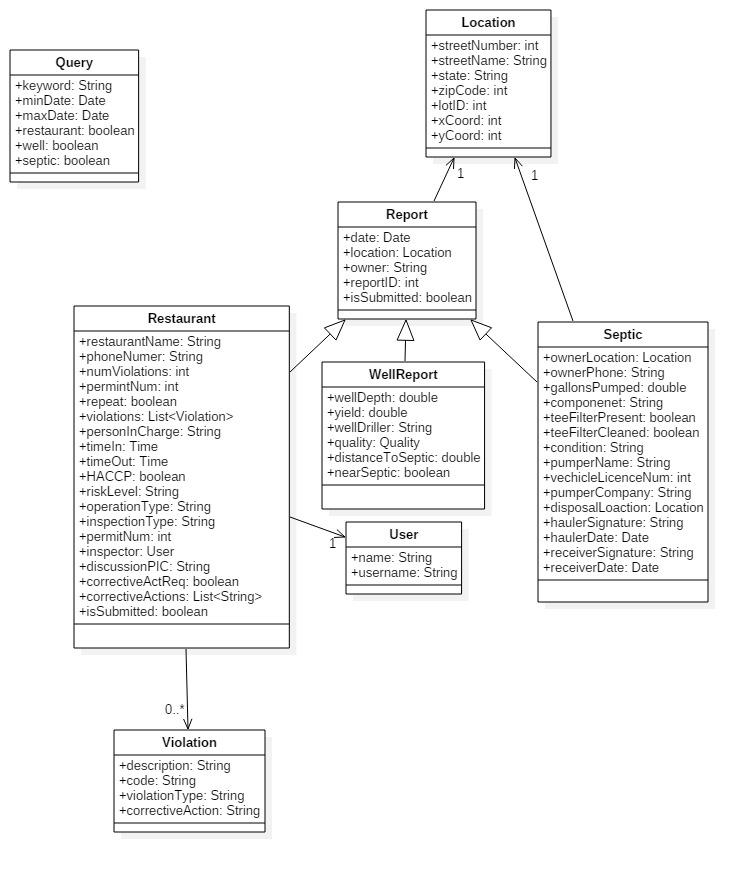
\includegraphics[width=6in,height=7in]{uml.jpg}
\end{figure}

\subsection[SYSTEM IMPLEMENTATION]{\selectlanguage{english}\rmfamily\bfseries\color{black}
SYSTEM IMPLEMENTATION}
{\selectlanguage{english}\rmfamily\color{black}
Health-e will be written in HTML5, CSS and Javascript. We will use the Ionic Framework to deploy the application for iOS and Android simultaneously. Ionic utilizes AngularJS and Sass to offer libraries for mobile-optimized HTML, CSS, and Javascript components. Additionally, we will be using the Ionic Material library for an advanced UI for our app. All classes and functions described in this section will be written in Javascript and will utilize these libraries.
}
\subsubsection{Class Definitions}
\begin{itemize}
\item Report - Superclass for Restaurant, Well and Septic classes. Contains most basic report/form information.
\item Restaurant - Subclass of Report. Contains all fields pertaining to Restaurant Form input.
\item Well -  Subclass of Report. Contains all fields pertaining to Well  Form input.
\item Septic - Subclass of Report. Contains all fields pertaining to Septic Form input.
\item Location - Specific information pertaining to where a report takes place.
\item User - References the user/inspector that is logged into the system and submitting a restaurant report.
\item Violation - Specifics to the type of restaurant violation including a text description.
\item Query - Contains ability to search for past submitted forms by report type, date, and keywords.
\end{itemize}
\subsubsection{Function Descriptions}
All classes will have getter and setter methods to give access to the many variables. These functions will be public so information about the reports can be accessed anywhere.

\clearpage\section[USER INTERFACE DESIGN]{\selectlanguage{english}\rmfamily\bfseries\color{black}
[USER INTERFACE DESIGN}

\subsection[DESCRIPTION OF THE USER INTERFACE]{\selectlanguage{english}\rmfamily\bfseries\color{black}
DESCRIPTION OF THE USER INTERFACE}
{\selectlanguage{english}\rmfamily\color{black}
Describe the functionality of the system from the users perspective. Explain how the user
will be able to use your system to complete all the expected features and the feedback
information that will be displayed for the user.
}

\subsubsection[Browsing and Search]{\selectlanguage{english}\rmfamily\bfseries\color{black}
Browsing and Search}
{\selectlanguage{english}\rmfamily\color{black}
Introduction to design document.
}

\subsubsection[Form Entry]{\selectlanguage{english}\rmfamily\bfseries\color{black}
Browsing and Search}
{\selectlanguage{english}\rmfamily\color{black}
Introduction to design document.
}

\subsubsection[Delayed Upload]{\selectlanguage{english}\rmfamily\bfseries\color{black}
Browsing and Search}
{\selectlanguage{english}\rmfamily\color{black}
Introduction to design document.
}

\subsection[FOR FIRST TIME USERS]{\selectlanguage{english}\rmfamily\bfseries\color{black}
FOR FIRST TIME USERS}
{\selectlanguage{english}\rmfamily\color{black}
Describethefunctionality of thesystem from the users perspective. Explain howtheuser
will be able to use your system to complete all the expected features and the feedback
information that will bedisplayedfor theuser.
}

\subsection[FOR RETURNING USERS]{\selectlanguage{english}\rmfamily\bfseries\color{black}
FOR RETURNING USERS}
{\selectlanguage{english}\rmfamily\color{black}
Describethefunctionality of thesystem from the users perspective. Explain howtheuser
will be able to use your system to complete all the expected features and the feedback
information that will bedisplayedfor theuser.
}

\subsection[SCREEN IMAGES]{\selectlanguage{english}\rmfamily\bfseries\color{black}
SCREEN IMAGES}
{\selectlanguage{english}\rmfamily\color{black}
Display screenshots showingtheinterfacefrom theusers perspective. Thesecan be handdrawn
or youcan use an automateddrawing tool. Just make them as accurateas possible.
(Graph paper workswell.)
}

\subsection[SCREEN OBJECTS \& ACTIONS]{\selectlanguage{english}\rmfamily\bfseries\color{black}
SCREEN OBJECTS \& ACTIONS}
{\selectlanguage{english}\rmfamily\color{black}
A discussion of screen objects andactions associatedwith thoseobjects.
}

\end{document}
